\chapter{Entwicklung}
In diesem Kapitel wird die Entwicklung des Prototypen beschrieben.
Der Prototyp ist ein GraphQL-Service welcher mit .NET 6 und der Zuhilfenahme der Bibilothek HotChocolate entwickelt wurde.
Desweiteren wird auf die von HotChocolate bereitgestellten Entwicklerhilfsmittel eingegangen.


\section{Anwendungsszenario}
% Der Anwendungsfall des Prototypen lässt sich wie folgt beschreiben:
% Da die Verwaltungen von Büchern und dazugehörige Autoren und Bewertungen ein aufwändiges Verfahren ist soll 
Die Auswahl eines neuen Buches ist oftmals ein sehr schwieriges Unterfangen.
Bei der Entscheidungsfindung helfen oft Bewertungen von Lesern die das jeweilige Buch schon gelesen haben.
Demnach soll eine Bücher-Bewertungsplattform geschaffen werden.
Diese Plattform ermöglicht es Benutzern Bücher zu bewerten und Informationen über Bücher, Autoren oder Bewertungen einzusehen.
% Benutzer, mit mehr Rechten als reinen Benutzerrechen, haben zudem die Möglichkeit die zusätzlich benötigten Entitäten 
Weiters sollen Benutzer in der Lage sein sich im System zu registrieren und anzumelden.
Angemeldete Benutzer haben, je nach ihren Benutzerrollen, Möglichkeiten im System verwaltete Entitäten zu Erstellen, zu Bearbeiten oder zu Löschen.

\section{Datenbankschema}
Das in der folgenden Abbildung dargestellte ER-Diagram beschreibt die dem Prototypen zu Grunde liegende Datenbank.

\begin{figure}[H]
    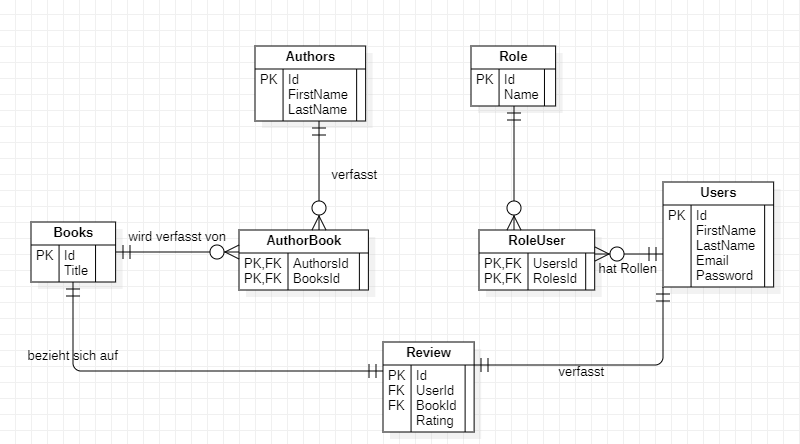
\includegraphics[width=\textwidth]{pics/ER-Diagram.png}
    \caption{Datenbankschema}
\end{figure}


\section{Architektur}
Der Prototyp wurde mit der für REST-APIs üblichen Drei-Schicht-Architektur umgesetzt.
Die Geschäftslogikschicht und Datenbankzugriffsschicht wurden dabei so entwickelt, dass sie eigentlichen Implementierungen je nach Bedarf einfach ausgetauscht werden können.
Auf die Geschäftslogik wird in den Unterkapiteln Query, Mutation und Subscription näher eingegangen. Die Datenbankzugriffsschicht wird im Kapitel Entity Framework näher erläutert.
\newline

\textit{API:}
Die API die einzige Schnittstelle des Systems zur Außenwelt.
\newline

\textit{Geschäftslogik:}
Die Geschäftslogik bildet dabei die Logik der Server-Applikation ab.
\newline

\textit{Datenbankzugriff:}
Die darunterliegende Datenbankzugriffsschicht ermöglicht, den darüberliegenden Schichten, CRUD-Operationen auf die angeforderten Daten auszuführen.
\newline

\begin{figure}[H]
    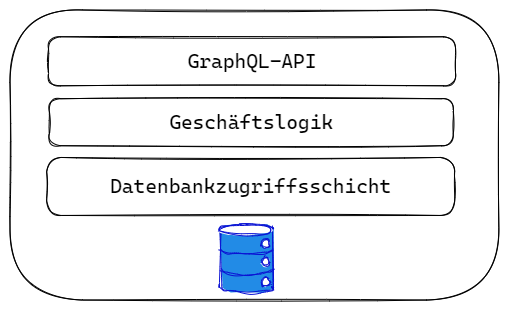
\includegraphics[width=\textwidth]{pics/architecture.png}
    \caption{Drei-Schicht-Architektur}
\end{figure}

\section{Hot Chocolate}
Der GraphQL-Service wurde mit dem Framework \textit{Hot Chocolate} umgesetzt.
Bei Hot Chocolate handelt es sich um einen Open Source GraphQL-Server welche 

\subsection{Entwurf Schema}

\section{Entity Framework}
Die Datenbankzugriffsschicht wurde mit dem \textit{Entity Framework} umgesetzt.
Das Entity Framework ist ein \textit{Object Relational Mapper}, es ermöglicht Entwicklern den Fokus auf eine höhere Abstraktionsebene zu legen.


\section{Querys}
\subsection{Pagination und Sorting}

\section{Mutations}

\section{Subscriptions}

\section{Authentifizierung und Autorisierung}

\begin{figure}[H]
    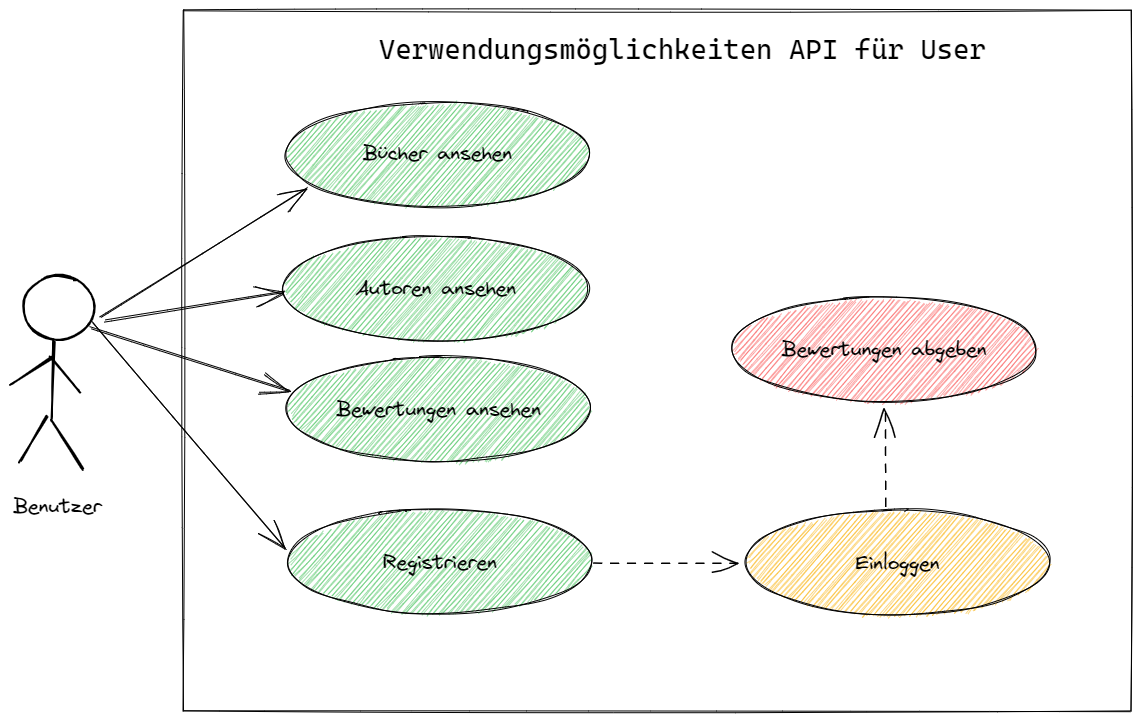
\includegraphics[width=\textwidth]{pics/UseCaseUser.png}
    \caption{Rechte User.}
\end{figure}

\begin{figure}[H]
    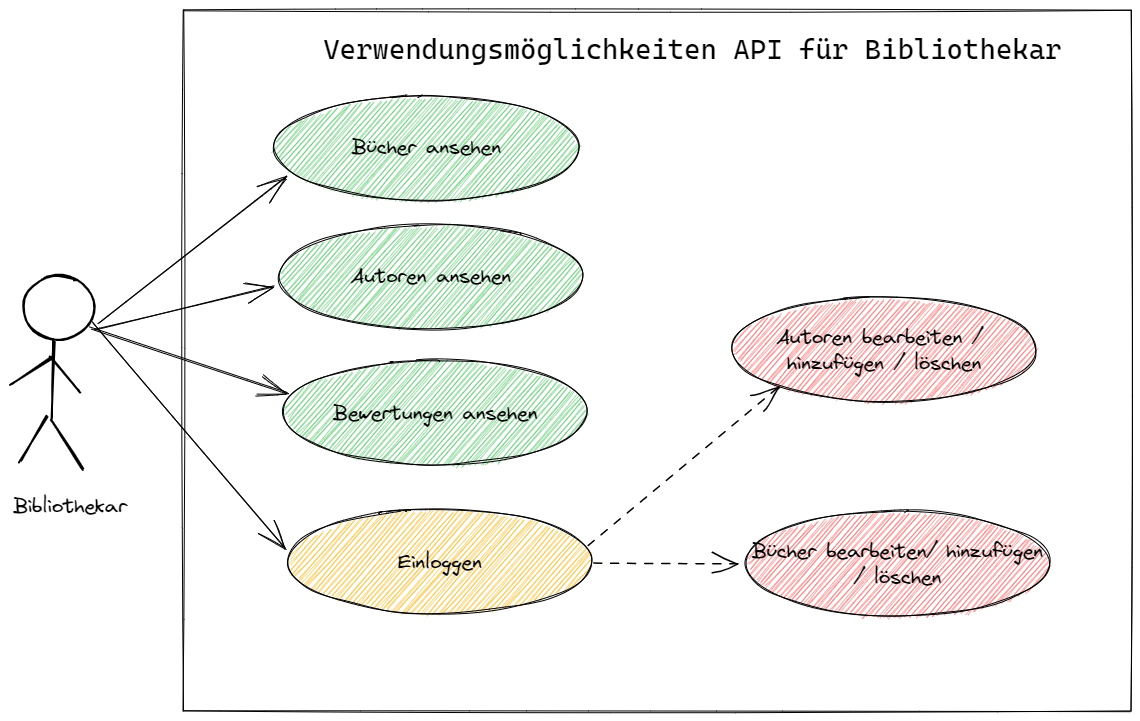
\includegraphics[width=\textwidth]{pics/UseCaseLibrarian.png}
    \caption{Rechte Bibliothekar.}
\end{figure}

\begin{figure}[H]
    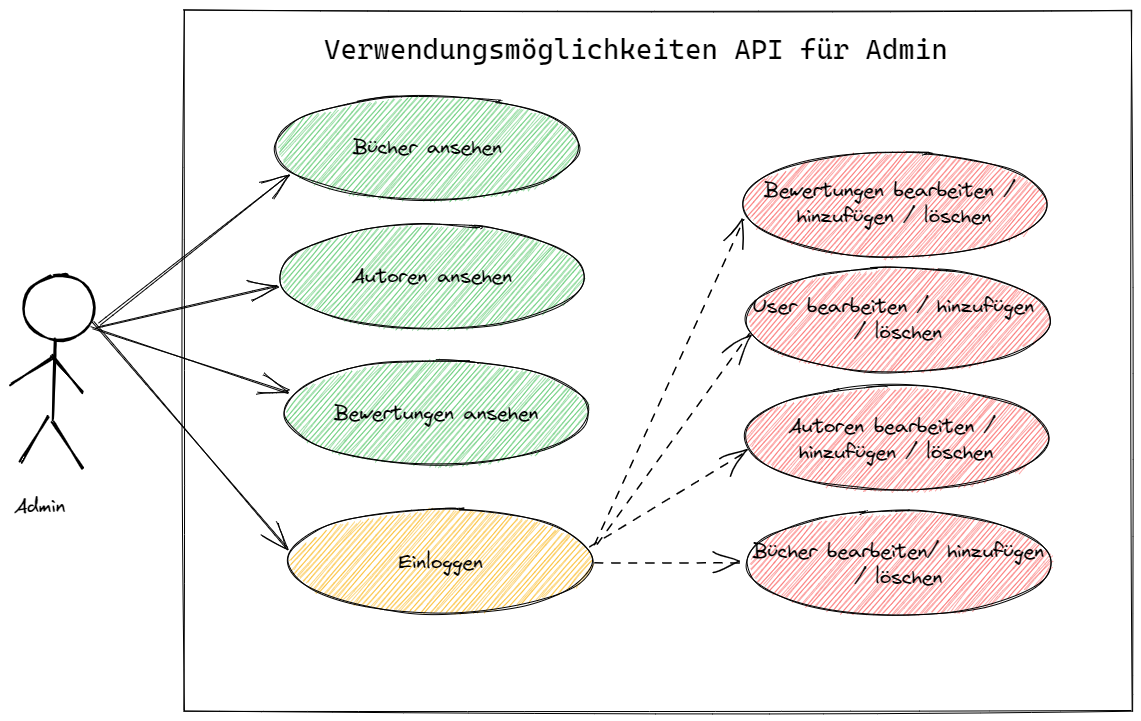
\includegraphics[width=\textwidth]{pics/UseCaseAdmin.png}
    \caption{Rechte Admin.}
\end{figure}

\section{Entwicklertools}
\subsection{GraphiQL}
\section{1 + n Problem}
\section{Fehlermanagement}
\section{Pagination}
\section{Caching}

